\clearpage
\newgeometry{margin=1cm}
\thispagestyle{empty}
\begin{landscape}
\begin{table}[t!]
\caption{Cost of safety guarantees}
\label{tbl-safety-cost}
    \begin{tabular}{lrrrrrrrrrrrrrrr} % UPDATED 20180305
    \toprule
                                        & B.sort     &  H.sort    & Bin.Search & XXTEA      & MD5        & RC5        & FFT        & Outlier    & LEC        & CoreMark   & MoteTrack  & HeatCalib  & HeatDetect & \makebox[0.2mm]{} &   average \\
    \midrule
    \midrule
    \multicolumn{10}{l}{EXECUTED BYTECODE INSTRUCTIONS (\% of total executed bytecode instructions)} \\
    Array element/object field STORES   &       18.0 &        7.8 &        0.0 &        2.9 &        4.5 &        1.5 &        6.1 &        5.8 &        3.7 &        2.6 &       10.0 &        1.4 &        4.7 &                   &       5.3 \\
    Array element/object field LOADS    &       18.0 &       15.9 &        7.1 &        8.6 &        6.2 &        6.4 &        7.0 &       10.7 &        7.9 &       11.6 &       21.4 &        4.1 &        9.8 &                   &      10.4 \\
    \multicolumn{10}{l}{PERFORMANCE OVERHEAD VS NATIVE C (\% of native C)} \\
    unsafe                              &      101.2 &       88.5 &       65.2 &       57.6 &       45.7 &       19.5 &       17.7 &       75.7 &       84.6 &       97.0 &      156.3 &       30.5 &       73.4 &                   &      70.2 \\
    safe writes                         &      247.5 &      153.9 &       65.2 &       68.2 &       60.3 &       22.2 &       30.3 &      128.4 &      118.4 &      124.0 &      266.1 &       33.9 &       91.3 &                   &     108.4 \\
    safe reads and writes               &      393.9 &      287.8 &      151.7 &      100.0 &       80.3 &       33.4 &       43.0 &      226.6 &      179.8 &      202.2 &      445.1 &       43.9 &      126.9 &                   &     178.0 \\
    \multicolumn{10}{l}{PERFORMANCE OVERHEAD VS UNSAFE VM (\% of unsafe AOT)} \\
    safe writes                         &       72.7 &       34.7 &        0.0 &        6.7 &       10.0 &        2.3 &       10.7 &       30.0 &       18.3 &       13.7 &       42.8 &        2.6 &       10.3 &                   &      22.4 \\
    safe reads and writes               &      145.5 &      105.7 &       52.4 &       26.9 &       23.7 &       11.6 &       21.5 &       85.9 &       51.6 &       53.4 &      112.7 &       10.3 &       30.9 &                   &      63.3 \\
    \multicolumn{10}{l}{CODE SIZE OVERHEAD VS NATIVE C (\% of native C)} \\
    unsafe                              &      118.6 &      100.0 &      112.3 &       55.1 &       54.9 &      121.8 &        2.5 &      110.5 &       88.6 &       50.7 &      117.1 &      -17.2 &      107.7 &                   &      78.7 \\
    safe writes                         &      125.4 &      105.4 &      112.3 &       56.2 &       55.7 &      125.3 &        5.0 &      118.9 &       94.3 &       54.5 &      125.4 &      -16.4 &      114.7 &                   &      82.8 \\
    safe reads and writes               &      132.2 &      113.4 &      117.8 &       60.1 &       59.1 &      132.3 &        8.0 &      123.2 &      102.9 &       61.8 &      145.3 &      -13.9 &      118.5 &                   &      89.3 \\
    \multicolumn{10}{l}{CODE SIZE OVERHEAD VS UNSAFE VM (\% of unsafe AOT)} \\
    safe writes                         &        3.1 &        2.7 &        0.0 &        0.7 &        0.5 &        1.6 &        2.4 &        4.0 &        3.0 &        2.5 &        3.8 &        1.0 &        3.4 &                   &       2.3 \\
    safe reads and writes               &        6.2 &        6.7 &        2.6 &        3.2 &        2.7 &        4.7 &        5.4 &        6.0 &        7.6 &        7.4 &       13.0 &        4.0 &        5.2 &                   &       5.9 \\
    \bottomrule
    \end{tabular}
\end{table}
\end{landscape}
\clearpage
\restoregeometry


\section{The cost of safety}
\label{sec-evaluation-safety}

The advantage of using a VM to provide safety is that the necessary checks are easy to do, compared to native code, and most can be done at translation time. This leads to both a very modest increase in VM complexity due to the safety checks, and a lower run-time overhead. 
% would be nice to get code size for Harbor and t-kernel.

\subsection{Run-time cost}
\label{sec-evaluation-run-time-cost}

\begin{figure}
\centering
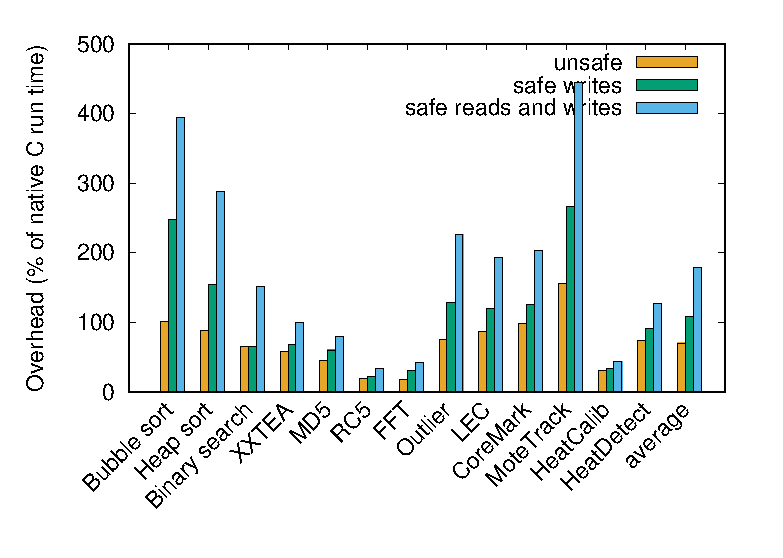
\includegraphics[width=\mygraphsize]{safety-cost.eps}
\caption{Overhead increase due to safety checks}
\label{fig-safety-cost-per-benchmark}
\end{figure}

\begin{figure}
\centering
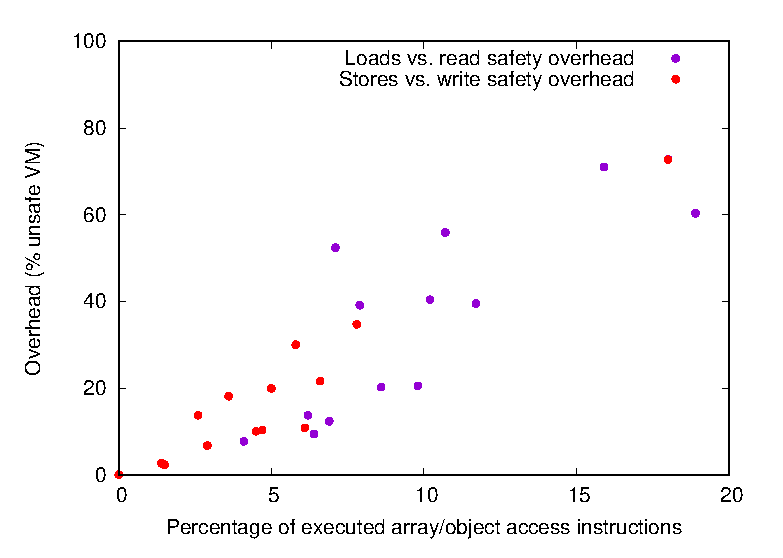
\includegraphics[width=\mygraphsize]{safety-ld-st-percentage-vs-overhead.eps}
\caption{Percentage of array/object load/store instructions and cost of read/write safety}
\label{fig-safety-ld-st-percentage-vs-overhead}
\end{figure}

\begin{figure}
\centering
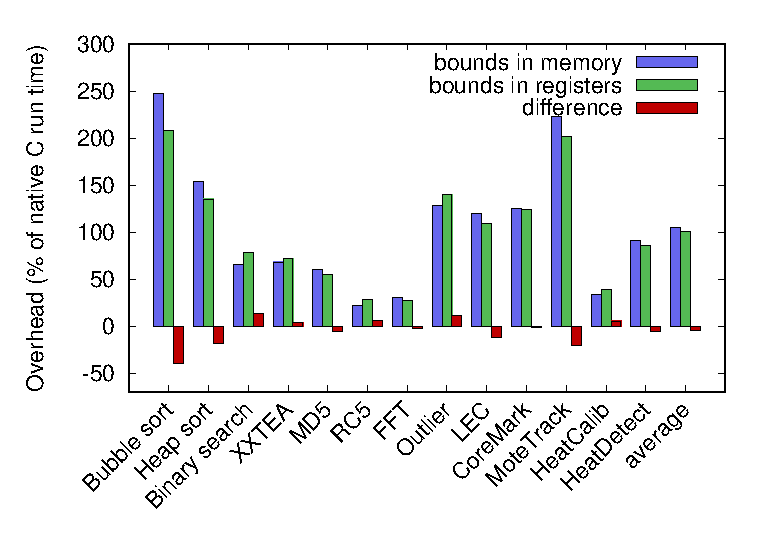
\includegraphics[width=\mygraphsize]{safety-cost-diff-using-regs.eps}
\caption{Comparison of safety cost with heap bounds in memory or registers}
\label{fig-safety-cost-memory-or-registers}
\end{figure}

Table \ref{tbl-safety-cost} shows the increase in performance and code size overhead as a result of the run-time safety checks for our 12 benchmarks. The performance overhead is also shown in Figure \ref{fig-safety-cost-per-benchmark}. The baseline here is the unsafe version of our VM, which is on average 70.2\% slower than native C. Adding write checks is sufficient to satisfy our guarantee that no malicious code can corrupt the state of the VM. This increases the average overhead to 108.4\% of native C, corresponding to a 22.4\% increase in run time compared to the unsafe VM.

The cost of the run-time safety checks depends greatly on the benchmark we run. Most checks are done at translation time, including writes to local and static variables. The only check that adds significant run-time overhead is check \ref{chk-memory-access-within-heap}, which checks the target of an object field or array write is within the bounds of the heap.

Thus, the run-time overhead is determined by the number of object or array accesses a benchmark does. The percentage of these is shown in the first part of Table \ref{tbl-safety-cost}. Since \mybench{bubble sort} has by far the highest percentage of array writes, at 18\% of all executed bytecode instructions, it also incurs the highest overhead from adding write safety, and slows down by 72.7\%. \mybench{Binary search} on the other hand, which does no writes at all, is unaffected. As usual \mybench{CoreMark}, being a large benchmark with a mix of operations, is somewhere in the middle. The correlation between the percentage of array and object writes, and the slowdown compared to the unsafe version is shown in Figure \ref{fig-safety-ld-st-percentage-vs-overhead}.

\subsubsection{Safe reads}
Next we consider read safety. Up to this point the VM only checks the application cannot \emph{write} to memory it is not supposed to write to, however, it may still \emph{read} from any location.

The recently published Meltdown and Spectre vulnerabilities in desktop CPUs can be exploited by malicious code to read from anywhere in memory, exposing both kernel's and other applications private data, which may contain sensitive information such as authentication tokens, passwords, etc. This sent OS vendors rushing to release patches, which early report suggest may cause a performance penalty of up to 11\% \cite{Simakov:2018wp}.

Whether this is also a problem on a sensor node depends on the scenario. If the VM or other tasks contain sensitive information, then this may need to be protected. However, in many sensor node applications the node may only be running a single application, and the VM does not contain any state that would be useful to an attacker. In these cases, write safety will be sufficient.

Adding read safety to our VM is trivial: instructions to load local and static variables are already protected since they use the same code to access a variable as the store instructions. For heap access, we simply add the same call to \mycode{heapcheck} to the \mycode{GETARRAY} and \mycode{GETFIELD} instructions just before the actual read.

Figure \ref{fig-safety-cost-per-benchmark} shows the cost of providing read safety is higher than write safety. Most applications read from an array or object much more frequently than they write to them. As a result, our VM with read and write safety turned on slows down by 63\% on average, corresponding to a 178\% slowdown over native C. In addition to the sort benchmarks, \mybench{MoteTrack} also suffers greatly from adding read safety, since it spends 21\% of its instructions reading from the objects and arrays, mostly from the RSSI signature database. \mybench{RC5} is the fastest benchmark, since it not only does relatively few array reads and writes, but also spends a large amount of time on expensive variable bit shifts, which have identical performance in both C and AOT compiled versions. The result is a slowdown of only 33\% compared to native C for the fully safe version.

\subsubsection{Keeping heap bounds in registers}
In Section \ref{sec-safety-heap-access} several alternatives for the heap bounds check were considered, one of which is to keep the bounds in dedicated registers to avoid having to fetch them from memory for each check. Here we evaluate this choice.

Having the bounds in registers would reduce the cost of the check from 22 to 14 cycles, reducing the overhead of safety checks by $8/22 \approx 36\%$. However, this uses 4 registers which we cannot use for stack caching.

To estimate how this would affect performance, the benchmarks were run using the unsafe VM, with the number of registers available to the stack cache reduced by 4. Since this does not affect the number of heap accesses, we then added the observed overhead for safety checks, reduced by 36\%.

Figure \ref{fig-safety-cost-memory-or-registers} shows the overhead for our chosen approach with the heap bounds in memory, compared to the expected overhead when the heap bounds are stored in registers. For some benchmarks such as \mybench{bubble sort} and \mybench{MoteTrack}, the savings in heap bounds checks outweighs the reduced effectiveness of the stack cache. But the improvement in performance is relatively small, and for other benchmarks the reverse is true, showing minor slowdowns when heap bounds are kept in registers. On average the benchmarks are quite balanced, as is the larger \mybench{CoreMark} benchmark.

As future work we may consider using some basic statistics, such as the percentage of array write instructions and average stack depth, to choose one of the two options on a per-method basis. But as usual there is a tradeoff, in this case VM size and complexity, which may not be worth the effort given the relatively small gains.

\subsection{Code-size cost}
Next, we examine the cost of safety in terms of code size. This comes in two parts: increased VM complexity and size, and an increase in the code it generates.

Most of our checks are not more complex than comparing two integers, and rejecting or terminating the application if a condition is not met. The most complex part is deciding the stack effects of instructions to guard against stack under- or overflow. This comes in the form of a table that encodes the effects of most instructions, and some specialised code to analyse a handful of instructions without fixed effect. In total, the increase in VM size for our safe version is a modest 1776 bytes.

As we can see in Table \ref{tbl-safety-cost}, the size of the code the VM generates increases by only 2.3\% for write only safety and 5.9\% when reads are also protected. Since many checks occur at translation time, most instructions produce exactly the same native code in the safe version of our VM. The exceptions are \mycode{INVOKEVIRTUAL} and \mycode{INVOKEINTERFACE}, which now contain the expected stack effects to realise check \ref{chk-invokevirtual-stack-effects-match}, and the array and object write instructions \mycode{PUTFIELD} and \mycode{PUTARRAY}, that emit a single extra \mycode{CALL} instruction the \mycode{heapcheck} routine. Since these instructions are both relatively rare, and already generate a larger than average block of native instructions, the total effect on code size is limited.

\subsection{Comparison to native code alternatives}
As discussed in Section \ref{sec-state-of-the-art-safety}, several non-VM approaches have been proposed to guarantee safety on a sensor node. Two of these, \emph{t-kernel} \cite{Gu:2006ww} and Harbor \cite{Kumar:2007ge}, allow the node to guarantee safety independent of the host. Both target the Mica family of sensor nodes, which use the same ATmega128 CPU used by CapeVM. In this section we compare them to CapeVM and consider the question whether a VM is a good way to provide safety.

\emph{t-kernel} reports a slowdown of between 50 and 200\%, which is roughly in the same range as CapeVM. However both \emph{t-kernel} and CapeVM provide additional advantages. In \emph{t-kernel}'s case a form of virtual memory, and for the VM platform independence. This makes them hard to compare, but we note that while the performance of both systems is similar, \emph{t-kernel}'s code size overhead is much higher at a 6-8.5x increase, limiting the size of programmes that can be loaded onto the device.

A better comparison is possible for Harbor, which only provides safety. Harbor uses three benchmarks to evaluate performance: writing arbitrary data to an array to mimick copying a buffer of sensor data, and the \mybench{outlier detection}, and 16-bit \mybench{FFT} benchmarks also used in the rest of CapeVM's evaluation. The size of the data used for the first two is not specified in the paper, but since it mentions they work on sensor data and the ATmega CPU has 13-bit analog-to-digital converters, we use 16-bit data for these benchmarks as well.

As mentioned before, the \mybench{FFT} benchmark is taken from the Harbor sources \cite{sos-operating-system}, and \mybench{outlier detection} implemented as described in the paper. The \mybench{array writes} benchmark is implemented as a loop that fills an array of 256 elements with an arbitrary number, as shown in Listing \ref{lst-fill-array}.


\begin{listing}
\begin{minted}{java}
    for (short i = 0; i < NUMBERS; i++) {
        numbers[i] = (short)1;
    }
\end{minted}
\caption{Array writes benchmark (8-bit version)}
\label{lst-fill-array}
\end{listing}

\begin{table}
\caption{Comparison of overhead in Harbor and CapeVM}
\label{tbl-safety-overhead-harbor}
    \begin{tabular}{lrrrrrrr} % UPDATED 20180316
    \toprule
    Benchmark    & \makebox[3mm]{} & \multicolumn{3}{c}{CapeVM overhead} & \makebox[2mm]{} & \multicolumn{2}{c}{Harbor overhead} \\
    \\
                 &                 & VM      & + safety checks & = safe VM   &                 & current & hypothetical              \\
    \midrule
    \midrule
    Array writes &                 & 182.8\% & 268.7\%       & 451.5\%   &                 & 1230\%  & 416\%                     \\
    Outlier      &                 & 75.8\%  & 52.7\%        & 128.5\%   &                 & 690\%   & 234\%                     \\
    16-bit FFT   &                 & 17.7\%  & 12.6\%        & 30.3\%    &                 & 380\%   & 129\%                     \\
    \bottomrule
    \end{tabular}
\end{table}



The resulting overhead is shown in Table \ref{tbl-safety-overhead-harbor}. Filling an array is a hard case for safe CapeVM since consecutive array writes are expensive for two reasons: (i) it results in repeated executions of the \mycode{PUTARRAY} instruction, which calculates the target address for each write, while native code can slide a pointer over the array, and (ii) each of these writes will trigger a call to \mycode{heapcheck}.

CapeVM incurs overhead both related to the VM, and because of the added run-time safety checks, while for Harbor all overhead is due to safety checks. Still, CapeVM's total overhead of 451.5\% is much lower than Harbor's 1230\%.

While CapeVM is more than twice as fast as Harbor for this benchmark, the comparison is not entirely fair. Harbor lists the cycle overhead for all of its 5 run-time protection primitives. We assume that without any function calls, only the 'Write access check' is relevant to this benchmark, which takes 65 cycles. In contrast, CapeVM's \mycode{heapcheck} routine only takes 22 cycles.

The difference is due to Harbor's more fine grained protection, which allows it to grant access to any aligned block of 8 bytes to the application, while CapeVM's protection is more coarse. If Harbor could be modified to use a similar check, its overhead could potentially be reduced to $1230 / 65 * 22 \approx 416\%$, slightly faster than CapeVM's total overhead. However, it is not clear from the paper whether Harbor's architecture could support such a coarse-grained check since it requires all application data that needs run-time write checks to be in a single block of memory.

While this shows CapeVM achieves a performance comparable to even a hypothetical optimised version of Harbor, the \mybench{array writes} benchmark does not highlight the advantage of using a VM to provide safety because it spends most of its time writing to an array, for which both approaches insert a run-time check. However, the VM can verify writes to local and static variables to be safe at translation time, while the Harbor sources \cite{sos-operating-system} show that its verifier requires \emph{all} stores to go through the run-time write access check. The authors do note that static analysis of the code could reduce the number of checks, but that this would come at the cost of a significantly more complex verifier.

CapeVM's \emph{total} overhead for the \mybench{array writes} benchmark is slightly higher than the hypothetical optimised Harbor, but the overhead due to safety checks is lower because CapeVM does not need to check writes to the index variable \mycode{i}. This advantage should be more pronounced in code with more frequent writes to local variables, which is exactly the case for the more realistic \mybench{outlier detection} and \mybench{FFT} benchmarks. Even with the faster memory access check, Harbor's overhead would be at 234\% or 129\% respectively, while our VM is significantly faster at only 128.5\% or 30.3\%.
